\documentclass[border=12pt]{standalone}
\usepackage{amsmath, amssymb}
\usepackage{tikz}
\usetikzlibrary{arrows.meta, positioning, shapes.geometric, fit, backgrounds, calc}

\begin{document}

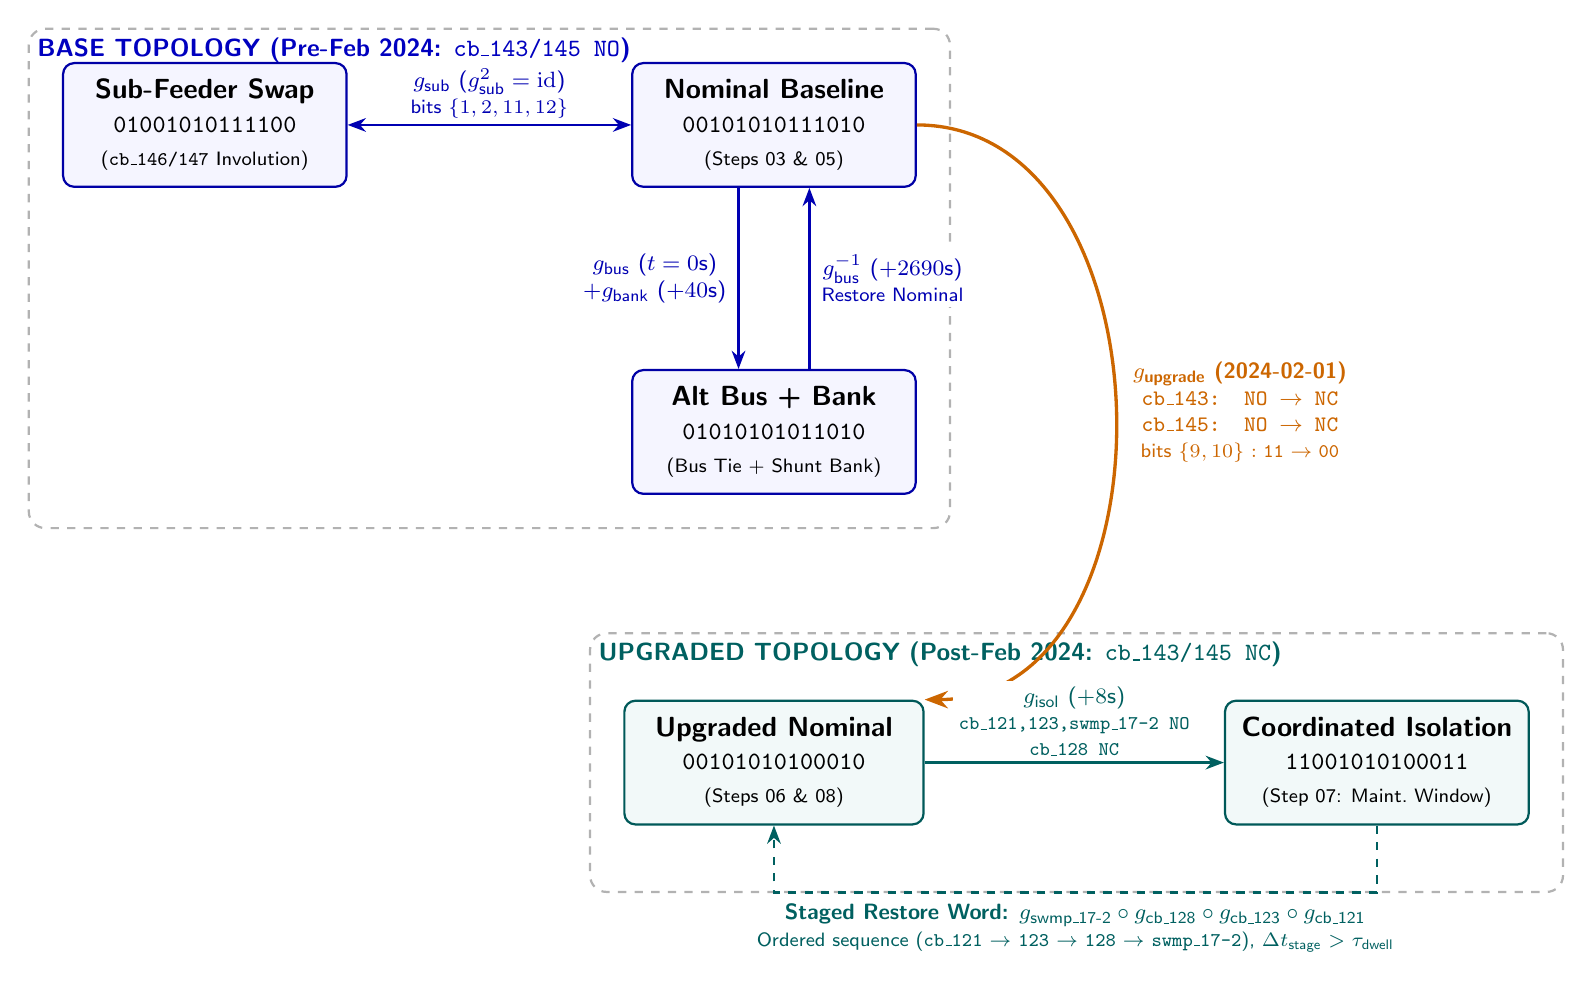
\begin{tikzpicture}[
    >=Stealth,
    node distance=1.8cm and 3.4cm,
    every node/.style={font=\sffamily},
    state/.style={
        rectangle,
        rounded corners=4pt,
        draw=blue!65!black,
        thick,
        fill=blue!4,
        align=center,
        minimum width=3.6cm,
        minimum height=1.35cm,
        inner sep=6pt
    },
    upgstate/.style={
        rectangle,
        rounded corners=4pt,
        draw=teal!70!black,
        thick,
        fill=teal!5,
        align=center,
        minimum width=3.8cm,
        minimum height=1.35cm,
        inner sep=6pt
    },
    gen/.style={
        font=\footnotesize\sffamily,
        align=center,
        fill=white,
        inner sep=2pt
    },
    regime/.style={
        rounded corners=6pt,
        draw=gray!60,
        dashed,
        thick,
        inner sep=12pt
    }
]

% =========================================================================
% REGIME 1: BASE TOPOLOGY (Pre-Feb 2024: cb_143/145 NO)
% =========================================================================
\node[state] (nom) {
    \textbf{Nominal Baseline} \\
    \texttt{\small 00101010111010} \\
    \scriptsize (Steps 03 \& 05)
};

\node[state, left=3.6cm of nom] (sub) {
    \textbf{Sub-Feeder Swap} \\
    \texttt{\small 01001010111100} \\
    \scriptsize (\texttt{cb\_146/147} Involution)
};

\node[state, below=2.3cm of nom] (alt) {
    \textbf{Alt Bus + Bank} \\
    \texttt{\small 01010101011010} \\
    \scriptsize (Bus Tie + Shunt Bank)
};

% Transitions in Base Topology
\draw[<->, thick, blue!70!black] (sub) -- node[above, gen] {
    $g_{\text{sub}}$ ($g_{\text{sub}}^2 = \mathrm{id}$) \\
    \scriptsize bits $\{1,2,11,12\}$
} (nom);

\draw[->, thick, blue!70!black] ([xshift=-0.45cm]nom.south) -- node[left, gen, xshift=-2pt] {
    $g_{\text{bus}}$ ($t=0\text{s}$) \\
    $+ g_{\text{bank}}$ ($+40\text{s}$)
} ([xshift=-0.45cm]alt.north);

\draw[->, thick, blue!70!black] ([xshift=0.45cm]alt.north) -- node[right, gen, xshift=2pt] {
    $g_{\text{bus}}^{-1}$ ($+2690\text{s}$) \\
    \scriptsize Restore Nominal
} ([xshift=0.45cm]nom.south);

% =========================================================================
% REGIME 2: UPGRADED TOPOLOGY (Post-Feb 2024: Step 06 & 08)
% =========================================================================
\node[upgstate, below=2.6cm of alt] (upg) {
    \textbf{Upgraded Nominal} \\
    \texttt{\small 00101010100010} \\
    \scriptsize (Steps 06 \& 08)
};

\node[upgstate, right=3.8cm of upg] (isol) {
    \textbf{Coordinated Isolation} \\
    \texttt{\small 11001010100011} \\
    \scriptsize (Step 07: Maint.\ Window)
};

% Structural Upgrade Transition (Base -> Upgraded)
\draw[->, very thick, orange!80!black] (nom.east) to[out=0, in=0, looseness=1.15] node[right, gen, xshift=4pt] {
    \textbf{$g_{\text{upgrade}}$ (2024-02-01)} \\
    \texttt{cb\_143: NO $\to$ NC} \\
    \texttt{cb\_145: NO $\to$ NC} \\
    \scriptsize bits $\{9,10\}: \texttt{11} \to \texttt{00}$
} (upg.north east);

% Coordinated Isolation Transition
\draw[->, thick, teal!75!black] (upg.east) -- node[above, gen] {
    $g_{\text{isol}}$ ($+8\text{s}$) \\
    \scriptsize \texttt{cb\_121,123,swmp\_17-2 NO} \\
    \scriptsize \texttt{cb\_128 NC}
} (isol.west);

% Staged Restore Path (4-step ordered generator word)
\draw[->, thick, dashed, teal!75!black] (isol.south) -- ++(0,-0.85) -| node[below, pos=0.25, gen, yshift=-2pt] {
    \textbf{Staged Restore Word:} $g_{\text{swmp\_17-2}} \circ g_{\text{cb\_128}} \circ g_{\text{cb\_123}} \circ g_{\text{cb\_121}}$ \\
    \scriptsize Ordered sequence (\texttt{cb\_121} $\to$ \texttt{123} $\to$ \texttt{128} $\to$ \texttt{swmp\_17-2}), $\Delta t_{\text{stage}} > \tau_{\text{dwell}}$
} (upg.south);

% =========================================================================
% BACKGROUND REGIME CONTAINERS
% =========================================================================
\begin{pgfonlayer}{background}
    \node[regime, fit=(sub)(nom)(alt), label={[anchor=north west, font=\small\bfseries\sffamily, text=blue!75!black]north west:BASE TOPOLOGY (Pre-Feb 2024: \texttt{cb\_143/145 NO})}] (box1) {};
    \node[regime, fit=(upg)(isol), inner ysep=24pt, label={[anchor=north west, font=\small\bfseries\sffamily, text=teal!75!black]north west:UPGRADED TOPOLOGY (Post-Feb 2024: \texttt{cb\_143/145 NC})}] (box2) {};
\end{pgfonlayer}

\end{tikzpicture}

\end{document}

